\documentclass{elsinta}
\usepackage{url}

% --- Memasukkan Data Dokumen Menggunakan Perintah Baru ---
\projectcode{EL2}
\documentname{\LiteraturesStandardsTitle}
\documenttitle{Teknik Elektro - Sistem Informasi Tugas Akhir}
\capstonetitle{Teknik Elektro - Sistem Informasi Tugas Akhir}
\shortname{  ELSINTA} 
\documentnumber{TA2526.01.099}
\revisionnumber{03}
\publicationdate{22 September 2025}

\revdatefooter{03/10/2025}
% --- Memasukkan Data Halaman Pengesahan (Halaman 2) ---
\currentpage{2} % Halaman yang sedang dicetak

% Data Tim
\ketuatimnama{Mahasiswa 1}
\ketuatimnim{12345678}

\anggotanamaI{Mahasiswa 2}
\anggotanimI{12345678}

\anggotanamaII{Mahasiswa 3}
\anggotanimII{12345678}


% Data Dosen
\pembimbingInama{Dosen 1}
\pembimbingInip{12345678 123456 1 123}

\pembimbingIInama{Dosen 2}
\pembimbingIInip{12345678 123456 1 123}


% Tanggal Pengesahan
\approvaldate{22 September 2025}

\begin{document}

% Panggil perintah untuk membuat halaman sampul
\coverpage
% Pindah ke Halaman Baru
\newpage

% Membuat Halaman Pengesahan (Halaman 2)
% \approvalpage

% Lanjut ke halaman proposal
% \newpage

% ======================================
% Bagian Konten Proposal Dimulai di Sini
% ======================================

% Mengatur ulang nomor halaman dan gaya halaman
\clearpage
\pagenumbering{arabic}
\setcounter{page}{1} 
\pagestyle{myfooter} % Ganti dari 'plain' ke 'myfooter'

% Atur margin standar (Opsional, jika Anda ingin margin isi berbeda dari sampul)
% \newgeometry{left=4cm, right=3cm, top=3cm, bottom=3cm} 
% Catatan: Perintah \newgeometry memerlukan paket 'geometry' yang sudah ada di cls.

\tableofcontents
\newpage
\section*{\docsumary}
Document Summary merupakan ringkasan yang hanya membahas isi dari dokumen capstone yang sedang dikerjakan, bukan keseluruhan proyek capstone. Bagian ini menjelaskan secara singkat tujuan, ruang lingkup, dan pokok pembahasan dari dokumen tersebut. Misalnya, pada dokumen EL1, ringkasan berfokus pada latar belakang, identifikasi masalah, dan lain-lain sesuai isi dari EL1.  Penulisan dilakukan secara padat dan jelas agar pembaca dapat langsung memahami inti dari dokumen tersebut tanpa mengaitkannya dengan bagian atau dokumen capstone lainnya.
\newpage

\section{\ProjectBenchmarkTitle}
% Bagian ini menyajikan tinjauan komprehensif terhadap solusi, proyek, penelitian, atau paten terdahulu yang relevan dengan topik proyek Sistem Monitoring Getaran dan Suhu Motor Induksi. Tujuannya adalah untuk memahami kondisi teknologi terkini, mengidentifikasi celah (gap), dan menegaskan improvisasi dari proyek yang diusulkan.

\subsection{\PrevProjectsTitle}
% Subbab ini membahas sistem atau proyek yang telah diimplementasikan, baik secara komersial maupun sebagai prototipe, yang memiliki fungsi serupa.

    \begin{figure}[b!]
        \centering
        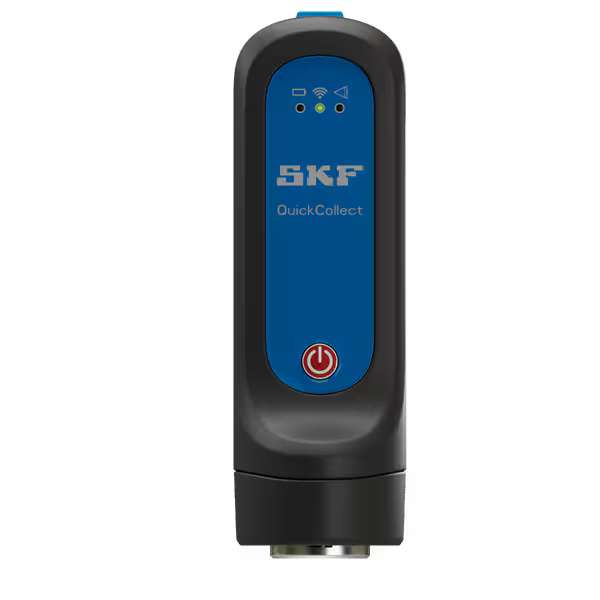
\includegraphics[width=0.5\textwidth]{image/doc/cmdt391.png}
        \caption{Sensor QuickCollect CMDT 391}
        \label{fig:fishbone}
    \end{figure}

\subsubsection*{Identifikasi Solusi Terdahulu:}
\begin{enumerate}
    \item \textbf{SKF QuickCollect CMDT392 (Komersial):}
    \begin{enumerate}
        \item \textbf{Fitur:} Sensor getaran, kondisi bearing, dan suhu terpadu yang mampu diintegrasikan dengan aplikasi pemantauan cloud terkoneksi android dan iOS (cite).
        \item \textbf{Kelebihan:} Maksimum percepatan ($50g$), rentang frekuensi internal sensor ($\leq f \leq 10000Hz$), \textit{sample rate} ($256\leq sr \leq 32768$) sampel \cite{2.1.1}, aplikasi mudah dioperasikan user.
        \item \textbf{Kekurangan:} Harga sangat mahal yang berkisar $Rp26.000.000,00$ hingga $Rp50.000.000,00$, solusi berlebihan untuk sistem skala UMKM.
        \item \textbf{Celah produk:} Mengembangkan solusi pemantauan motor induksi minim biaya yang dilengkapi aplikasi pemantauan remote.
    \end{enumerate}
    \item \textbf{Siemens SIDRIVE IQ (Komersial):}
    \begin{enumerate}
        \item \textbf{Fitur:} Jasa IoT industri dalam pemantauan kondisi, \textit{preventive maintenance}, analisis kegagalan reaktif \cite{2.1.2}.
        \item \textbf{Kelebihan:} Sistem analitik berbasis IoT dengan dukungan kendali jarak jauh, Motor Damage Detection System, Pemodelan numerik berbasis IoT cloud \cite{2.1.2}.
        \item \textbf{Kekurangan:} Sistem SIDRIVE IQ dilakukan melalui platform cloud Siemens, biaya implementasi tinggi sehingga tidak cocok untuk industri tingkat UMKM, ekosistem yang bersifat vendor lock-in, algoritma analistik yang bersifat proprietary.
        \item \textbf{Celah produk:} Menyajikan sistem pemantauan kondisi motor induksi berbasis sensor getaran dan sensor suhu yang bersifat low-cost sehingga mampu diakses bisnis skala UMKM. Mengembangkan model yang mampu dilatih menggunakan data motor lokal sehingga mampu mendeteksi kerusakan dan melakukan klasifikasi kerusakan pada motor induksi.
    \end{enumerate}
\end{enumerate}
 
\subsection{\RelResearchPatentsTitle}
% Subbab ini mengulas penelitian ilmiah dan paten yang telah dipublikasikan terkait teknologi atau metodologi yang akan digunakan.
\begin{enumerate}
    \item \textbf{Paten:} Metode Pemantauan Getaran Rotating Equipment secara Real-Time dengan Pemrosesan FFT menggunakan Mikrokontroler.
    \begin{enumerate}
        \item \textbf{Studi:} Paten ini menyajikan metode pemantauan getaran dan mikrokontroler ESP32. Data akuisisi sensor diolah oleh mikrokontroler dengan memanfaatkan algoritma \textit{fast-fourier transform} (FFT) untuk menghasilkan spektrum frekuensi dan gelombang waktu.
        \item \textbf{Relevansi dengan  Proyek ini:} Proyek ini memanfaatkan algoritma FFT dan Mikrokontroler ESP32 sebagai fungsi transfer yang akan digunakan untuk menganalisa dan mengklasifikasikan kondisi motor.
        \item \textbf{Kontribusi  ELSINTA:} Mengimplementasikan FFT pada motor induksi, visualisasi data hasil algoritma FFT secara efisien via aplikasi berbasis cloud, yang mengimplementasikan sistem algoritma diagnostik.
    \end{enumerate}
    \item \textbf{Riset:} \textit{Health Monitoring of Induction Motor through Vibration Analysis} \cite{1.1.17}
    \begin{enumerate}
        \item \textbf{Studi:} Paper ini membahas mengenai pengukuran sinyal getaran melalui metode Non-Destructive Testing (NDT) dengan menggunakan mikrokontroler Arduino R3 dan sensor akselerometer ADXL335 pada motor induksi 3-fasa.
        \item \textbf{Relevansi dengan  Proyek ini:} Proyek ini akan mengadopsi metodologi VAT dengan memanfaatkan accelerometer MEMS seperti ADXL335 atau ADXL345.
        \item \textbf{Kontribusi  ELSINTA:} Mengimplementasikan sensor suhu thermocouple sebagai parameter pemantauann alternatif pada sistem pemantauan motor induksi.
    \end{enumerate}
    
    % \item \textbf{Penelitian tentang Fusi Sensor (Suhu + Getaran) untuk Diagnosis Motor Induksi:}
    % \begin{enumerate}
    %     \item \textbf{Studi:} Penelitian \cite{}  mengonfirmasi bahwa fusi sensor suhu dan getaran meningkatkan akurasi diagnosis kerusakan motor secara signifikan dibandingkan penggunaan parameter tunggal. Suhu efektif mendeteksi overload dan kerusakan kumparan stator, sedangkan getaran efektif untuk kerusakan mekanis. Kombinasi keduanya mencapai tingkat deteksi >90\%.
    %     \item \textbf{Relevansi dengan  Proyek ini:} Proyek ini mengimplementasikan fusi sensor dengan menempatkan sensor suhu pada stator (winding) dan bearing housing, serta sensor getaran pada kedua sisi bearing.
    %     \item \textbf{Kontribusi  Proyek ini:} Mengembangkan algoritma logika aturan (rule-based system) yang menggabungkan data getaran (nilai RMS dan pola FFT) dan data suhu untuk menghasilkan rekomendasi tindakan pemeliharaan spesifik (misalnya: "Getaran tinggi + suhu normal → cek balancing rotor"; "Getaran normal + suhu tinggi → cek beban lebih atau pendinginan"). Sistem ini akan diperkenalkan sebagai fitur actionable insight yang belum banyak ditemukan pada prototipe penelitian sebelumnya.
    % \end{enumerate}
    % \item \textbf{Jurnal tentang Implementasi IoT untuk Predictive Maintenance:}
    % \begin{enumerate}
    %     \item \textbf{Studi:} Artikel oleh Mystkowski et al. (2022) dalam Sensors (MDPI) menunjukkan arsitektur IoT menggunakan ESP32 dan protokol MQTT efektif untuk pemantauan kondisi mesin pertanian secara real-time dengan delay rata-rata <500 ms. Platform Blynk dan ThingsBoard direkomendasikan untuk visualisasi dashboard karena kemudahan integrasi dengan ESP32.
    %     \item \textbf{Relevansi dengan  Proyek ini:} Proyek ini akan mengimplementasikan arsitektur serupa menggunakan ESP32 sebagai unit pemrosesan utama dan platform IoT open-source (Blynk atau ThingsBoard) untuk dashboard.
    %     \item \textbf{Kontribusi  Proyek ini:} Mendesain sistem IoT yang ramah pengguna dengan time-delay $\leq$ 1000 ms (sesuai target EL1) dan menyediakan dashboard visual yang secara jelas menampilkan kategori status motor (Normal/Warning/Danger) berdasarkan standar ISO 10816, serta grafik trend getaran dan suhu historis untuk analisis degradasi jangka panjang.
    % \end{enumerate}
\end{enumerate}

\section{\GapAnalysisTitle}
% Berdasarkan tolok ukur proyek pada bagian sebelumnya, subbab ini akan secara spesifik mengidentifikasi kesenjangan atau celah yang ada pada solusi/penelitian terdahulu. Analisis ini sangat penting untuk memvalidasi improvisasi yang dihasilkan proyek yang diusulkan, dengan menunjukkan bagaimana proyek ini akan mengisi celah-celah tersebut dan memberikan kontribusi yang berarti.

\subsection{\LimitationsTitle}
% Solusi-solusi  yang ada saat ini, baik produk komersial maupun prototipe hasil penelitian sebelumnya, memiliki beberapa keterbatasan kunci yang belum sepenuhnya teratasi. Contoh Keterbatasan:
\begin{enumerate}
    \item \textbf{Solusi terlalu mahal untuk UMKM:} Solusi yang ada saat ini seperti SKF CMDT391 dan layanan Siemens SIDRIVE IQ umumnya ditujukan untuk industri tingkat atas. 
    \item \textbf{Sistem pemantauan yang terbatas pada parameter tertentu:} Sebagian besar sistem pemantauan mesin dengan biaya investasi rendah hanya berfokus pada satu atau dua parameter utama.
    \item \textbf{Kurangnya sistem diagnostik cerdas:} Banyak sistem pemantauan yang hanya berfungsi sebagai alat akuisisi dan visualisasi data tanpa dibekali algoritma analisis lanjutan dalam mengidentifikasi jenis kerusakan.  
    \item \textbf{Visualisasi data yang kurang informatif dan tidak real-time:} Platform masih menyajikan data dalam bentuk angka mentah atau grafik yang susah dipahami oleh pengguna.
\end{enumerate}

\subsection{\ProjectContribsTitle}
% Sub-bab ini secara eksplisit mengidentifikasi dan mendokumentasikan \textbf{kontribusi} yang dihasilkan oleh Proyek Capstone ini. Contoh celah yang diisi oleh project:
\begin{enumerate}
    \item \textbf{Sistem Monitoring Motor Induksi Multi-Sensor Low-Cost Berbasis Sensor Getar dan Sensor Suhu:} Sistem terintegrasi yang tidak hanya mengukur getaran, tetapi juga memantau kondisi motor, arus, tegangan, dan kondisi lingkungan operasional.
    \item \textbf{Monitoring dan Visualisasi Real-Time Berbasis IoT:} Sistem menyediakan dashboard yang menampilkan data historis, tren parameter, dan status kesehatan motor.
    \item \textbf{Sistem Peringatan Dini:} Sistem mampu memberikan notifikasi ketika parameter operasional melewati ambang batas tertentu.
\end{enumerate}

\section{Standar dan Regulasi}
% Bagian ini menguraikan standar teknis, regulasi, dan aturan yang harus dipenuhi oleh proyek Sistem Monitoring Getaran dan Suhu Motor Induksi. Mematuhi standar menjamin kualitas, keamanan, dan interoperabilitas sistem, sementara mematuhi regulasi memastikan legalitas dan kepatuhan terhadap keselamatan kerja serta lingkungan.

\subsection{Standar Teknis}
% Standar teknis adalah pedoman yang diadopsi secara luas untuk memastikan konsistensi, keandalan, dan interoperabilitas komponen sistem.

% \subsubsection{ISO 20816-1:2016 1st ed.}
% \textbf{Penjelasan:} Panduan ini menetapkan kondisi dan prosedur pengukuran dan evaluasi getaran pada mesin rotating, non-rotating dan non-reciprocating. Panduan ini merujuk pada ISO 2954 mengenai getaran mekanik dari mesin rotating dan reciprocating, ISO 5348 mengenai getaran mekanik dan kejut mekanik, dan ISO 10817-1 mengenai sistem pengukuran getaran rotating shaft.

% \textbf{Penerapan pada proyek:} 
% \begin{enumerate}
%     \item Rentang frekuensi getaran harus menggunakan pengukuran \textit{broad-band} dengan rentang $1Hz\leq f\leq1000Hz$ berdasarkan panduan ISO 20816, dengan catatan disesuaikan dengan tipe mesin.
%     \item Penentuan tipe pengukuran getaran dibagi menjadi tiga jenis; pengukuran getaran pada bagian non-rotating, relative shaft, dan absolute shaft.
%     \item Parameter pengukuran yang digunakan dalam mendefinisikan getaran; \textit{vibration displacement} ($mm$), \textit{vibration velocity} ($mm/s$), \textit{vibration acceleration} ($m/s^2$)
%     \item Pergeseran getar dapat didefinisikan dengan beberapa parameter; \textit{maximum vibratory displacement} ($s_{max}$), \textit{peak-to-peak vibratory displacement} ($s_{(p-p)}$), dan \textit{maximum peak-to-peak vibratory displacement} ($s_{(p-p)max}$).
%     \item Posisi ukur diklasifikasikan menjadi bagian non-rotating dan rotating shaft berdasarkan panduan ISO 20816-1:2016.
% \end{enumerate}

% \subsubsection{ISO 13373-1:2002}
% \textbf{Penjelasan:} 
% % Perubahan pola getar pada motor induksi disebabkan oleh hal berikut; perubahan balance, perubahan alignment, wear atau damage pad journal atau bearing anti-friction, gear atau coupling defects, crack pada komponen kritis, operation transients, transient excitations pada mesin listrik, rubbing, mekanik longgar.
% ISO 13373-1 mencakup rekomendasi pada metode pengukuran, parameter pengukuran, pemilihan jenis dan lokasi transduser, pengumpulan data, kondisi operasi mesin, sistem pemantauan getaran, sistem pengkondisian sinyal, sistem interface pemrosesan data, pemantauan kontinyu dan periodik. Panduan ini merujuk pada ISO 1925 mengenai kosakata getaran mekanik, ISO 2041 mengenai kosakata getaran dan kejut mekanik, ISO 7919-1 mengenai getaran mekanik pada mesin non-reciprocating, serta ISO 10816-1 mengenai getaran mekanik.

% \textbf{Penerapan pada proyek:}
% \begin{enumerate}
%     \item Tipe sistem pemantauan kondisi getar terbagi menjadi sistem terinstal permanen, semi-permanen, dan portable.
%     \item Metode pengumpulan data dilakukan secara kontinyu dan/atau periodik.
%     \item Panduan program pemantauan kondisi seperti pada gambar ...
%     \item 
% \end{enumerate}

% \subsubsection{ISO 13373-2}
% \textbf{Penjelasan:}

% \textbf{Penerapan pada proyek:}


\subsubsection{ISO 10816-3:2009}
\textbf{Penjelasan:} ISO 10816-3:2009 mencakup  semua jenis motor listrik, termasuk motor induksi. Dokumen ini merujuk pada beberapa normatif, ISO 2041 mengenai getaran mekanik, kejut, dan pemantauan kondisi, ISO 2954 mengenai getaran mekanik mesin berputar, ISO 10817-1 mengenai sistem pengukuran getaran rotating shaft, dan ISO 20816-1 mengenai petunjuk umum pengukuran dan evaluasi getaran mesin.
Memberikan panduan spesifik untuk menilai tingkat keparahan getaran radial yang diukur pada rumah bantalan (\textit{bearing housings}) mesin industri secara \textit{in situ} \cite{iso10816_2009}. Standar ini berlaku untuk motor listrik dari semua jenis dengan daya di atas 15 kW dan kecepatan operasi antara 120 rpm hingga 15000 rpm \cite{iso10816_2009_bsi}. Dua kriteria evaluasi disediakan: kriteria pertama mempertimbangkan besaran getaran yang teramati, sedangkan kriteria kedua mempertimbangkan perubahan besaran getaran dari waktu ke waktu \cite{iso10816_2009}.

\textbf{Penerapan pada Proyek:} 
Sistem akan mengukur nilai RMS kecepatan getaran (mm/s) pada \textit{bearing housing} motor. Nilai ini akan dibandingkan dengan tabel batasan ISO 10816-3 untuk motor induksi (Kelas II: motor dengan daya 15-300 kW; Kelas III: motor dengan daya >300 kW atau mesin dengan \textit{foundation} kaku). Hasilnya akan dikategorikan ke dalam:
\begin{itemize}
    \item \textbf{Zone A (Baik):} Getaran rendah, motor baru atau dalam kondisi sangat baik.
    \item \textbf{Zone B (Diizinkan):} Motor dapat beroperasi tanpa batasan.
    \item \textbf{Zone C (Kurang Baik):} Motor boleh beroperasi untuk waktu terbatas, perbaikan harus direncanakan.
    \item \textbf{Zone D (Berbahaya):} Getaran cukup parah menyebabkan kerusakan, hentikan motor sesegera mungkin.
\end{itemize}
Evaluasi ini berlaku untuk pengukuran pita lebar (\textit{broad-band measurements}) dalam kondisi operasi steady-state dan relevan untuk pemantauan operasional berkelanjutan maupun tidak berkelanjutan \cite{iso10816_2009_bsi}.

\textbf{Justifikasi:} Pemilihan ISO 10816-3 didasarkan pada rekomendasi pada dokumen EL1 (Analisis Bisnis, proposisi nilai poin 3) dan penggunaan standar ini secara luas di industri pemeliharaan mesin.

\subsubsection{IEEE 802.11-2020}
\textbf{Penjelasan:} Standar ini, yang dikeluarkan oleh \textit{Institute of Electrical and Electronics Engineers} (IEEE), mendefinisikan lapisan fisik (PHY) dan lapisan kontrol akses medium (MAC) untuk implementasi \textit{Wireless Local Area Network} (WLAN). Standar IEEE 802.11 merupakan fondasi teknologi Wi-Fi yang memungkinkan perangkat elektronik terhubung ke jaringan nirkabel \cite{ieee80211_2020}.

\textbf{Penerapan pada Proyek:} Modul Wi-Fi terintegrasi pada mikrokontroler ESP32 wajib memenuhi standar IEEE 802.11 b/g/n untuk memastikan perangkat dapat terhubung dengan \textit{access point} (router) yang tersedia di lingkungan laboratorium atau industri. Frekuensi operasi yang digunakan adalah 2.4 GHz, yang merupakan pita frekuensi umum untuk komunikasi WLAN.

\subsubsection{IEC 60034-1:2022}

\textbf{Penjelasan:} Standar internasional dari \textit{International Electrotechnical Commission} (IEC) ini merupakan bagian dari seri IEC 60034 yang membahas tentang mesin listrik berputar (\textit{rotating electrical machines}). Bagian pertama dari seri ini mencakup persyaratan umum, rating, performa, karakteristik operasional, dan metode pengujian untuk semua jenis mesin listrik berputar, termasuk motor induksi \cite{iec60034_2022}. Standar ini menjadi acuan global untuk menentukan batasan operasi aman motor listrik, termasuk batas kenaikan suhu berdasarkan kelas isolasi.

\textbf{Penerapan pada Proyek:} Digunakan untuk menentukan batasan suhu operasi motor induksi berdasarkan kelas isolasi (Kelas B: kenaikan suhu maksimum 80°C dengan suhu sekitar 40°C; Kelas F: kenaikan suhu maksimum 105°C dengan suhu sekitar 40°C). Sistem akan mengatur ambang batas peringatan (\textit{warning}) dan bahaya (\textit{danger}) berdasarkan rekomendasi IEC 60034-1. Penggunaan standar ini memastikan bahwa sistem monitoring yang dikembangkan selaras dengan praktik internasional dalam pemeliharaan mesin listrik.

\subsubsection{ISO/IEC 20922:2016 (Protokol MQTT)}

\textbf{Penjelasan:} Standar ini mendefinisikan protokol \textit{Message Queuing Telemetry Transport} (MQTT) versi 3.1.1, yang merupakan protokol komunikasi \textit{publish/subscribe} yang ringan (\textit{lightweight}), terbuka, sederhana, dan mudah diimplementasikan \cite{mqtt_2016}. Protokol ini dirancang khusus untuk lingkungan dengan keterbatasan sumber daya, seperti komunikasi \textit{Machine to Machine} (M2M) dan \textit{Internet of Things} (IoT), di mana \textit{code footprint} yang kecil dan bandwidth jaringan yang terbatas menjadi pertimbangan utama \cite{mqtt_2016}. MQTT berjalan di atas TCP/IP dan mendukung tiga tingkat \textit{Quality of Service} (QoS) untuk pengiriman pesan.

\textbf{Penerapan pada Proyek:} ESP32 akan mengirimkan data sensor (getaran, suhu, kecepatan, arus) ke \textit{broker} MQTT di \textit{cloud}. \textit{Dashboard} akan berlangganan (\textit{subscribe}) ke topik yang sama untuk menampilkan data secara \textit{real-time}. Penggunaan protokol MQTT menjamin efisiensi transmisi data dengan \textit{time-delay} minimal.

\subsubsection{ISO 9001:2015}

\textbf{Penjelasan:} Standar sistem manajemen mutu internasional ini menetapkan persyaratan untuk organisasi yang ingin memastikan konsistensi produk/layanan dan peningkatan kepuasan pelanggan melalui implementasi proses yang efektif \cite{iso9001_2015}. Standar ini bersifat generik dan dirancang untuk dapat diterapkan oleh semua organisasi, terlepas dari jenis, ukuran, atau produk/layanan yang mereka sediakan \cite{iso9001_sme}. Tujuh prinsip manajemen mutu menjadi dasar dari ISO 9001, termasuk fokus pada pelanggan, kepemimpinan, pendekatan proses, dan perbaikan berkelanjutan.

\textbf{Penerapan pada Proyek:} Meskipun proyek ini adalah prototipe, prinsip-prinsip ISO 9001 digunakan sebagai pedoman dalam proses:
\begin{itemize}
    \item \textbf{Dokumentasi:} Menyusun dokumentasi teknis dan manual pengguna yang lengkap (sesuai Tujuan Utama poin 4 pada EL1).
    \item \textbf{Pengujian:} Melakukan pengujian terstruktur (verifikasi, validasi, pengujian pengguna) dan mencatat hasilnya.
    \item \textbf{Perbaikan:} Menggunakan umpan balik dari pengguna untuk perbaikan iteratif sistem.
\end{itemize}
Pendekatan ini juga relevan dengan karakteristik organisasi kecil seperti tim proyek capstone, di mana komunikasi lebih sederhana dan langsung, namun sumber daya terbatas \cite{iso9001_sme}.

\subsection{Regulasi}

% Regulasi adalah aturan hukum yang wajib dipatuhi. Dalam konteks proyek pemantauan kondisi motor induksi, regulasi berikut relevan:

\subsubsection{Undang-Undang Nomor 30 Tahun 2009 tentang Ketenagalistrikan}

\textbf{Penjelasan:} Undang-undang ini mengatur tentang penyelenggaraan ketenagalistrikan di Indonesia, mencakup pembangkitan, transmisi, distribusi, dan pemanfaatan tenaga listrik \cite{uu30_2009}. Dalam pasal 2 ayat (1), undang-undang ini menetapkan asas-asas pembangunan ketenagalistrikan termasuk asas keamanan dan keselamatan, yang menjadi dasar hukum bagi seluruh kegiatan yang berkaitan dengan pemanfaatan tenaga listrik \cite{uu30_2009}. Selain itu, undang-undang ini juga mengatur persyaratan teknis instalasi listrik dan kewajiban untuk memastikan keselamatan operasional.

\textbf{Penerapan pada Proyek:}
\begin{itemize}
    \item Sistem pemantauan harus dipasang tanpa mengganggu operasi normal motor (\textit{non-intrusif}).
    \item Sensor suhu yang dipasang pada area bertegangan (stator) harus memiliki isolasi listrik yang memadai (menggunakan thermocouple dengan selubung isolasi atau sensor digital dengan isolasi).
    \item Seluruh instalasi kabel sensor harus terisolasi dengan baik dan tidak menimbulkan risiko sengatan listrik atau hubungan pendek (\textit{short circuit}).
    \item Pengujian sistem hanya boleh dilakukan oleh personel yang kompeten dan memahami risiko kelistrikan.
\end{itemize}

\subsubsection{Peraturan Menteri Ketenagakerjaan Nomor 5 Tahun 2018 tentang Keselamatan dan Kesehatan Kerja Lingkungan Kerja}

\textbf{Penjelasan:} Peraturan Menteri ini mengatur tentang Keselamatan dan Kesehatan Kerja (K3) Lingkungan Kerja, yang merupakan upaya perlindungan terhadap tenaga kerja dari faktor-faktor bahaya lingkungan di tempat kerja, termasuk faktor fisika (kebisingan, getaran, iklim kerja), faktor kimia, faktor biologi, faktor ergonomi, dan faktor psikologi \cite{permenaker5_2018}. Regulasi ini mewajibkan setiap tempat kerja untuk melakukan pengukuran dan pengendalian lingkungan kerja secara berkala, memastikan kondisi lingkungan kerja tetap berada di bawah Nilai Ambang Batas (NAB) yang ditetapkan.

\textbf{Penerapan pada Proyek:} Sistem pemantauan ini berkontribusi langsung pada pengendalian risiko dari kerusakan motor induksi yang dapat menyebabkan kecelakaan kerja (misalnya motor macet total, percikan api akibat korsleting, atau getaran berlebih yang merusak \textit{foundation}). Meskipun NAB getaran dalam Permenaker 5/2018 berfokus pada dampak getaran terhadap tubuh manusia (tangan-lengan atau seluruh tubuh), implementasi sistem \textit{early warning} pada motor induksi secara tidak langsung turut melindungi pekerja dari risiko kecelakaan akibat kegagalan mesin. Dengan sistem peringatan dini, tindakan pemeliharaan preventif dapat dilakukan sebelum kerusakan membahayakan pekerja atau lingkungan.

\subsubsection{Peraturan DJID (Direktorat Jenderal Infrastruktur Digital) tentang Sertifikasi Perangkat Telekomunikasi}

\textbf{Penjelasan:} Berdasarkan Peraturan Menteri Komunikasi dan Digital (KOMDIGI) Nomor 13 Tahun 2025, perangkat telekomunikasi yang beredar dan digunakan di Indonesia wajib memenuhi persyaratan teknis dan administratif yang ditetapkan, termasuk pengujian di laboratorium yang ditunjuk oleh DJID (dahulu dikenal sebagai SDPPI) \cite{sdppi_2025}. Persyaratan ini mencakup perangkat HKT (\textit{Handheld Terminal} seperti ponsel) dan non-HKT, termasuk perangkat yang menggunakan Wi-Fi atau Bluetooth \cite{sdppi_2025}. Pengujian meliputi aspek keselamatan listrik (Electrical Safety), kompatibilitas elektromagnetik (EMC), dan karakteristik frekuensi radio (RF).

\textbf{Penerapan pada Proyek:} Mikrokontroler ESP32 yang digunakan dalam proyek ini harus memiliki sertifikasi DJID (atau SDPPI) yang berlaku. Sertifikasi ini menjamin bahwa perangkat beroperasi dalam spektrum frekuensi yang diizinkan (2.4 GHz) dan tidak menyebabkan interferensi berbahaya dengan perangkat lain. Untuk penggunaan dalam lingk terbatas seperti prototipe penelitian di lingkungan akademik, ketentuan ini dapat dipenuhi dengan memastikan pembelian modul ESP32 dari distributor resmi yang telah memiliki sertifikasi.

\subsubsection{Standar Operasional Prosedur (SOP) Keselamatan Laboratorium ITERA}

\textbf{Penjelasan:} ITERA memiliki prosedur internal untuk keselamatan dan kesehatan kerja di lingkungan laboratorium, termasuk Laboratorium Teknik Elektro, Laboratorium Sistem Kendali, dan Laboratorium Konversi Energi. SOP ini mengacu pada peraturan perundang-undangan nasional serta standar keselamatan laboratorium pendidikan tinggi. Prosedur ini mencakup aturan penggunaan peralatan bertegangan, prosedur darurat, dan tata cara pelaporan insiden.

\textbf{Penerapan pada Proyek:}
\begin{itemize}
    \item Seluruh proses perakitan dan pengujian prototipe wajib mengikuti SOP ITERA yang berlaku.
    \item Pengujian dengan motor induksi yang terhubung ke sumber listrik (terutama motor 3 fasa) harus disaksikan oleh teknisi laboratorium atau dosen pembimbing.
    \item Prosedur \textit{Lock-Out/Tag-Out} (LOTO) harus diterapkan saat memasang sensor pada motor yang sedang tidak beroperasi, untuk memastikan motor tidak dapat dihidupkan secara tidak sengaja.
    \item Alat pemadam api ringan (APAR) harus tersedia di area pengujian.
\end{itemize}

\subsubsection{Standar Nasional Indonesia (SNI) terkait Motor Listrik}

\textbf{Penjelasan:} SNI merupakan standar yang ditetapkan oleh Badan Standardisasi Nasional (BSN) yang berlaku secara sukarela namun dapat diwajibkan melalui peraturan teknis. Untuk motor listrik, SNI 04-6958-2003 mengatur persyaratan umum motor induksi, meskipun dokumen yang tersedia menunjukkan bahwa SNI ini lebih berfokus pada aspek pelabelan untuk peralatan rumah tangga \cite{sni_6958_2003}. Dalam praktiknya, Indonesia sering mengadopsi standar internasional seperti IEC 60034 sebagai acuan teknis untuk mesin listrik berputar, termasuk motor induksi.

\textbf{Penerapan pada Proyek:} Proyek ini akan menggunakan motor induksi yang memenuhi standar keselamatan yang berlaku (setidaknya memiliki sertifikasi SNI jika tersedia di laboratorium, atau setara dengan standar internasional). Parameter ambang batas (suhu, getaran, arus) akan disesuaikan dengan rekomendasi SNI atau IEC 60034-1. Jika SNI spesifik untuk motor induksi berdaya rendah tidak tersedia, tim proyek akan mengacu pada standar internasional yang diakui secara global.
\section{\ReferencesTitle}
% Daftar pustaka ditulis sesuai standar IEEE, sebaiknya gunakan Citation tools seperti Mendeley, Zotero dll.  
% Contoh format IEEE:  
\renewcommand{\refname}{}      % Hapus judul default "Pustaka"
\bibliographystyle{IEEEtran} % Menggunakan style sitasi IEEE
\bibliography{pustaka}    % Memanggil file pustaka.bib





\section{\AbbrevTitle}

% longtable tidak menggunakan lingkungan table[] di sekitarnya.
% Perintah \begin{longtable} langsung menggantikan \begin{table}\begin{tabular}
\begin{longtable}{|p{4cm}|p{11cm}|} % Lebar kolom ditetapkan agar teks wrap
    \caption{Daftar Singkatan (Abbreviations)} \label{tab:abbreviations2} \\
    \hline
    \textbf{Abbreviation} & \textbf{Definition} \\
    \hline
    \endhead % Mengakhiri baris header yang akan diulang di setiap halaman
    
    \hline 
    \multicolumn{2}{|r|}{Lanjutan di halaman berikutnya...} \\ 
    \endfoot % Footer untuk semua halaman kecuali yang terakhir
    
    \hline
    \endlastfoot % Footer untuk halaman terakhir (kosong)

    % --- Isi Tabel ---
    IoT & Internet of Things \\
    \hline
    KPI & Key Performance Indicator \\
    \hline
    ROI & Return on Investment \\
    \hline
    WBS & Work Breakdown Structure \\
    \hline
    SWOT & Strengths, Weaknesses, Opportunities, Threats \\
    \hline
    BMC & Business Model Canvas \\
    \hline
    IEEE & Institute of Electrical and Electronics Engineers \\
    \hline
    ISO & International Organization for Standardization \\
    \hline
    G-MoCo & Gas Quality Monitoring and Controlling (Nama Proyek Anda) \\
    \hline
    CO & Carbon Monoxide \\
    \hline
    CH$_4$ & Methane (atau LPG) \\
    \hline
    PM2.5 & Particulate Matter 2.5 \\
    \hline
    
    % Tambahkan lebih banyak baris di sini untuk memicu pemisahan halaman
    % ... (Tambahkan entri lain jika tabel perlu memanjang)

\end{longtable}

% Tambahkan \newpage jika Anda ingin halaman isi dimulai di halaman berikutnya
% \newpage
% \section*{Pendahuluan}
% Di sinilah konten proposal Anda akan dimulai...

\end{document}